% Define Document Structure
\documentclass[a4paper]{article}

% Packages
\usepackage[english]{babel}
\usepackage[utf8]{inputenc}
\usepackage{amsmath}
\usepackage{graphicx}
\usepackage[colorinlistoftodos]{todonotes}
\usepackage{wrapfig}
\usepackage{array}
\usepackage{hyperref}
\usepackage{caption}
\usepackage{subcaption}
% Making my life easy with commands definition
% Need work on it and define more commands
\hypersetup{
	colorlinks=true,
	linkcolor=blue,
	filecolor=magenta,      
	urlcolor=cyan,
}



% Title Section
\title{Docker Documentation}
\author{Vishal Sharma \\ Data Science Intern}
\date{\today}



% Document Starts 
\begin{document}
	
% Build Title
\maketitle

% Section and Content
\section{Introduction}

\subsection{Docker as a platform}
% Content is from Wikipedia (cite Wiki)
Docker is a computer program that performs operating-system-level virtualization, also known as \textit{containerization}. Docker is used to run software packages called \textit{containers}. In a typical example use case, one container runs a web server and web application, while a second container runs a database server that is used by the web application. Containers are isolated from each other and bundle their own tools, libraries and configuration files; they can communicate with each other through well-defined channels. All containers are run by a single operating system kernel and are thus more lightweight than virtual machines. Containers are created from \textit{images} that specify their precise contents. Images are often created by combining and modifying standard images downloaded from repositories. \cite{wiki}

% Docker Stack image (wrap around text)
\begin{wrapfigure}{R}{0.5\textwidth}
	\centering
	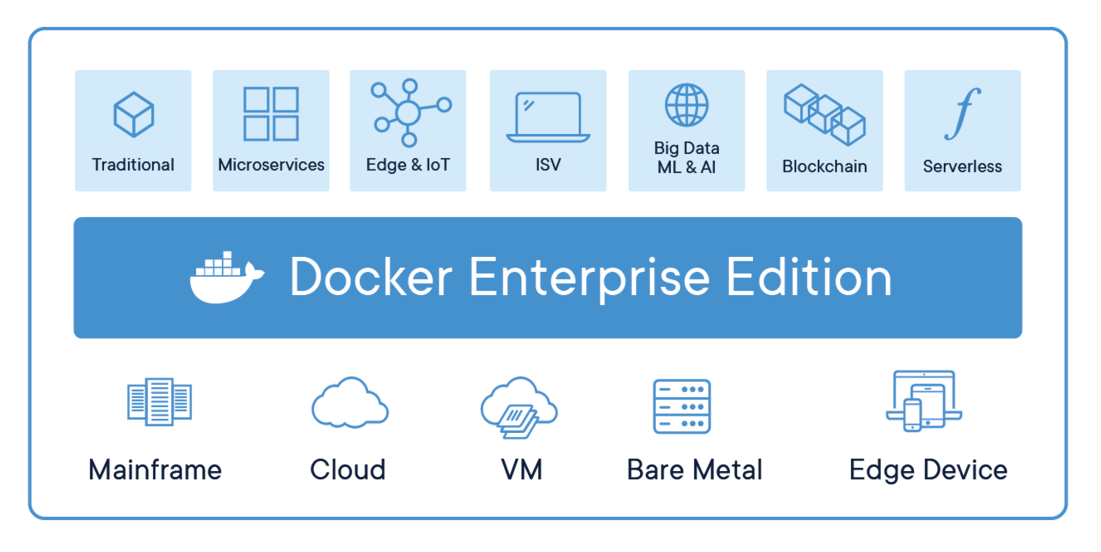
\includegraphics[width=0.50\textwidth]{./images/docker_stack.png}
	\caption{\label{fig:docker}Docker Stack}
\end{wrapfigure}

% Content is from Docker wensite (cite Docker webpage)
Docker increases productivity and reduces the time it takes to bring applications live, having the resources needed to invest in key digitization projects that cut across the entire value chain, such as application modernization, cloud migration and server consolidation. With Docker, we have the solution that helps manage the diverse libraries and infrastructure. 

The Docker Enterprise container platform delivers immediate value by reducing the infrastructure and maintenance costs of supporting existing application portfolio while accelerating time to market new solutions. \cite{docker} \footnote{https://github.com/docker}


\subsection{Docker vs VM}
A VM hypervisors, such as Hyper-V, KVM, and Xen, all are \textit{based on emulating virtual hardware}. That means they're fat in terms of system requirements.

Containers, however, use shared operating systems. This means they are much more efficient than hypervisors in system resource terms. Instead of virtualizing hardware, containers rest on top of a single Linux instance. This means you can leave behind the useless 99.9 percent VM junk, leaving you with a small, neat capsule containing your application. Therefore, with a perfectly tuned container system, you can have as many as four-to-six times the number of server application instances as you can using Xen or KVM VMs on the same hardware.

Another reason why containers are popular is they lend themselves to \textit{Continuous Integration/Continuous Deployment (CI/CD)}. This a DevOps methodology designed to encourage developers to integrate their code into a shared repository early and often, and then to deploy the code quickly and efficiently. Docker enables developers to easily pack, ship, and run any application as a lightweight, portable, self-sufficient container, which can run virtually anywhere. \textit{Containers gives you instant application portability}. Containers do this by enabling developers to isolate code into a single container. This makes it easier to modify and update the program. It also lends itself, as Docker points out, for enterprises to break up big development projects among multiple smaller, Agile teams using Jenkins, an open-source CI/CD program, to automate the delivery of new software in containers.


\begin{figure}
\centering
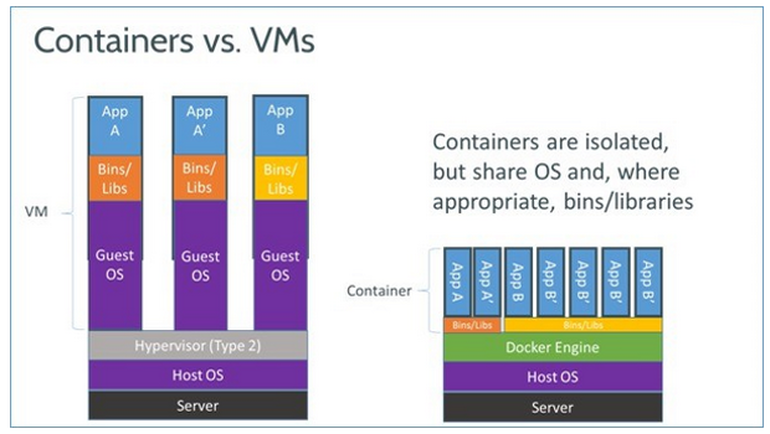
\includegraphics[width=10cm, height=5.5cm]{./images/docker-vm-container.png}
\caption{Containers vs VM's}
\end{figure}

% Define Setup steps for Docker
\section{Installation}
\subsection{Steps}
\begin{itemize}
	\item {Started with a restore point for system (in case I mess up something)}
	\item {There was an existing Docker version. It was older version and needed upgrade, could not upgrade because apt package was broken. No option except uninstall and re-install docker}
	\item {Ran into problems because of proxy}
	\item {Proxy setup on local GPU server and later in docker environment.}
	\item {Installation of Nvidia driver wapper around docker}
	\item {Tested Docker and CUDA. }
	\item {After a milestone, another system restore point. (You know why !! :) )}
	\item {Create docker image for deep learning container.}
	\item {Deleted other system restore except last.}
	\item {Docker Images created \textit{deep\_learning\_2.0} and \textit{deep\_learning\_3.0}}
\end{itemize}


% Define Packages Version
\subsection{Library Version}
\begin{center}
	\begin{tabular}{ l r }
		CUDA & 8.0 \\
		tensorflow-gpu & 1.4.0 \\
		Keras & 2.2.0 \\
		Theano & 1.0.2 \\
		pyTorch & 0.4.0 \\
		dlib & 19.15.0 \\
		cuDNN & 6.0 
	\end{tabular}
\end{center}



\subsection{Few helpful links for Installation}
\begin{itemize}
	\item {https://docs.docker.com/install/linux/docker-ce/\#ubuntu/uninstall-old-versions}
	\item {https://github.com/NVIDIA/nvidia-docker}
	\item {https://www.liquidweb.com/kb/how-to-install-docker-on-ubuntu-14-04-lts/]}
	\item {https://chunml.github.io/ChunML.github.io/project/Installing-NVIDIA-Docker-On-Ubuntu-16.04/}
	\item {https://github.com/ufoym/deepo}
	\item {https://github.com/floydhub/dl-docker}
	\item {\textit{Shell Script}: https://gist.github.com/katopz/7eb4d8c475ee61e18624f3787c33fc21}
\end{itemize}



\begin{thebibliography}{9}
	\bibitem{floydhub} 
	\textit{https://github.com/floydhub/dl-docker}. 
	
	\bibitem{wiki} 
	\textit{https://en.wikipedia.org/wiki/Docker\_(software)}
	
	\bibitem{docker}
	\textit{https://www.docker.com/why-docker}
	
	
	\bibitem{why_docker} 
	\textit{https://www.zdnet.com/article/what-is-docker-and-why-is-it-so-darn-popular/}
	
	\bibitem{pipeline_docker} 
	\textit{https://www.docker.com/sites/default/files/UseCase/\\RA\_CI\%20with\%20Docker\_08.25.2015.pdf}
\end{thebibliography}


\section{Commands}
% Display using Typewriter font 
\subsection{Few Docker Commands}
\begin{tabular} { >{\ttfamily}l  p{6.5cm} }
docker ps 						&	List the containers currently running on your machine.\\
docker ps -a 					&	List all the containers existing on your machine.\\
docker images 					&	List the images currently available on your machine.\\
docker rmi IMAGE\_ID 			&	Remove an image based on its image\_id .\\
docker pull USER:IMAGE\_NAME 	&	Download a given image to your machine.\\
docker run Container\_name 				&	Start a new container. It creates a new container of an image, and execute the container. You can create N clones of the same image. The command is: docker run IMAGE\_ID and not docker run CONTAINER\_ID \footnote{$https://bit.ly/2nz4mjJ$}\\
docker start CONTAINER\_ID 		&	Start an existing container based on its container\_id. Launches a container previously stopped. For example, if you had stopped a database with the command docker stop CONTAINER\_ID, you can relaunch the same container with the command docker start CONTAINER\_ID, and the data and settings will be the same.\\
docker start ALIAS  			&	Start an existing container based on its alias.\\
docker stop CONTAINER\_ID  		&	Stop a container based on its container\_id.\\
docker stop ALIAS 				&	Stop a container based on its alias.\\
docker rm CONTAINER\_ID 			&	Delete a container based on its container\_id. \\
docker rm ALIAS 				&	Delete a container based on its alias. \\
docker exec -it \\ CONTAINER\_ID bash&  Create an SSH session into a running container based on its container\_id. \\
docker exec -it ALIAS bash 		&	Create an SSH session into a running container based on its alias. \\
\end{tabular}

\begin{figure}[!h]
	\centering
	\begin{subfigure}{.5\textwidth}
		\centering
		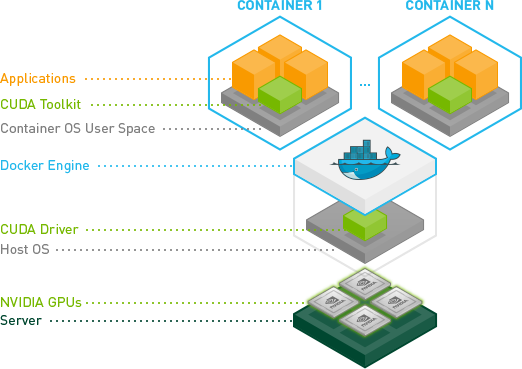
\includegraphics[width=5cm, height=4cm]{./images/nvidia_stack.png}
	\end{subfigure}%
	\begin{subfigure}{.5\textwidth}
		\centering
		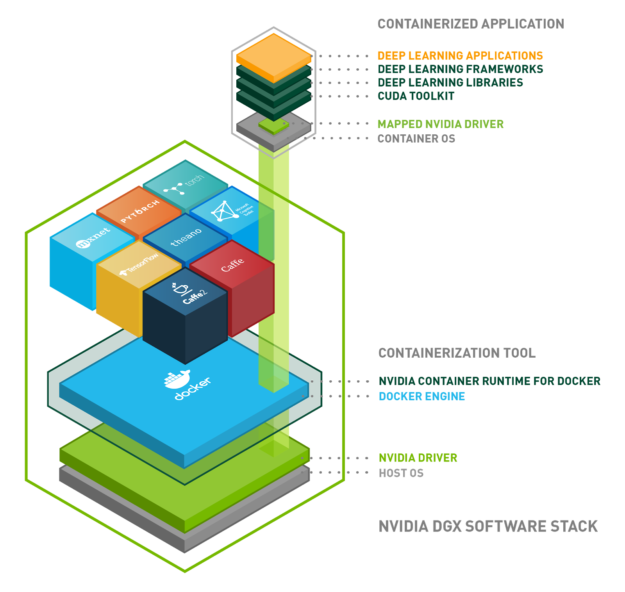
\includegraphics[width=5cm, height=4cm]{./images/docker.png}
	\end{subfigure}
	\caption{Deep Learning Stack using Docker}
	\label{fig:deep_learning}
\end{figure}

%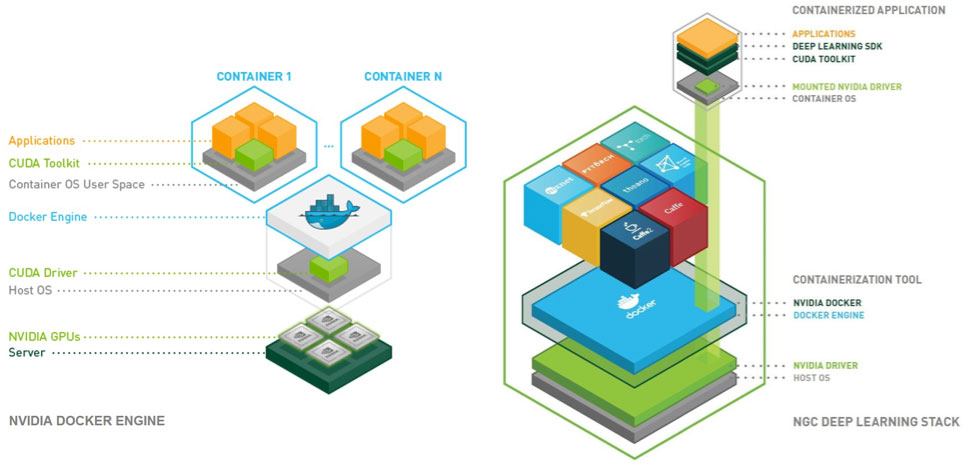
\includegraphics[width=10cm, height=5cm]{./images/nvidia_stack.jpg}
%\caption{}

% Content : https://github.com/floydhub/dl-docker
\subsection{Few Docker Parameters}
Parameter below uses examples and names from \cite{floydhub}  \\
\begin{tabular} { >{\ttfamily}p{3cm}  p{8.5cm} }

-it	& 		This creates an interactive terminal you can use to iteract with your container \\
-p 8888:8888 -p 6006:6006	& 		This exposes the ports inside the container so they can be accessed from the host. The format is -p $<$host-port$>$:$<$container-port$>$. The default iPython Notebook runs on port 8888 and Tensorboard on 6006 \\
-v /sharedfolder:/root\\/sharedfolder/ &			This shares the folder /sharedfolder on your host machine to /root/sharedfolder/ inside your container. Any data written to this folder by the container will be persistent. You can modify this to anything of the format -v /local/shared/folder:/shared/folder/in/container/. See \href{https://github.com/floydhub/dl-docker#docker-container-persistence}{Docker container persistence} \\
bash	& 		This provides the default command when the container is started. Even if this was not provided, bash is the default command and just starts a Bash session. You can modify this to be whatever you'd like to be executed when your container starts. For example, you can execute docker run -it -p 8888:8888 -p 6006:6006 floydhub/dl-docker:cpu jupyter notebook. This will execute the command jupyter notebook and starts your Jupyter Notebook for you when the container starts \\

-t              & Allocate a pseudo-tty \\
-i              & Keep STDIN open even if not attached \\
-e             & Set environment variable \\
\end{tabular}


\subsection{Multi GPU Sharing}
GPU isolation is achieved through a container environment variable called \\ NVIDIA\_VISIBLE\_DEVICES. Devices can be referenced by index (following the PCI bus order) or by UUID (refer to the \href{https://github.com/nvidia/nvidia-container-runtime#nvidia_visible_devices}{Docker documentation}).

\begin{verbatim}
Sample Command:

Split in two 
+ sudo nvidia-docker run --runtime=nvidia -e NVIDIA_VISIBLE_DEVICES=0,1
deep_learning_2.0 nvidia-smi
+ sudo nvidia-docker run --runtime=nvidia -e NVIDIA_VISIBLE_DEVICES=2,3 
deep_learning_2.0 nvidia-smi

Using all 4 GPU
+ sudo nvidia-docker run --runtime=nvidia -e NVIDIA_VISIBLE_DEVICES=0,1,2,3
deep_learning_2.0 nvidia-smi
\end{verbatim}




\vspace{45pt}
\textbf{Possible Values:}
\vspace{5pt}

\begin{tabular} { >{\ttfamily}l  p{6.5cm} }
0,1,2, GPU-fef8089b …: 		&	a comma-separated list of GPU UUID(s) or index(es).\\
all: 						&	all GPUs will be accessible, this is the default value in our container images.\\
none: 						&	no GPU will be accessible, but driver capabilities will be enabled.\\
void or empty or unset: 	&	nvidia-container-runtime will have the same behavior as runc.\\
\end{tabular}


\raggedright
\begin{verbatim}
#######################
# TESTING GPU Sharing #
#######################
\end{verbatim}
Started a docker container with GPU 0 and 1. Checking available GPU's using 
\begin{verbatim}
nvidia-smi
\end{verbatim}
\centering
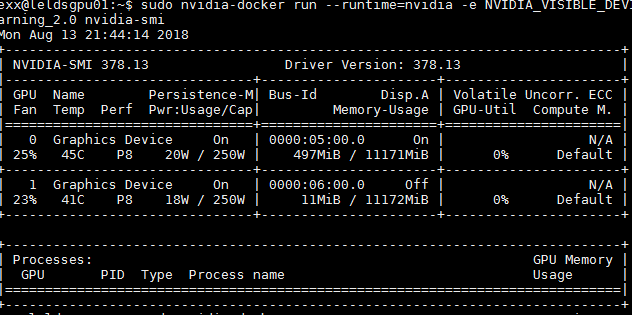
\includegraphics[width=10cm, height=5cm]{./images/gpu_0.PNG}

\raggedright
Started another docker container with GPU 2 and 3. Checking available GPU's using 
\begin{verbatim}
nvidia-smi
\end{verbatim}
\centering
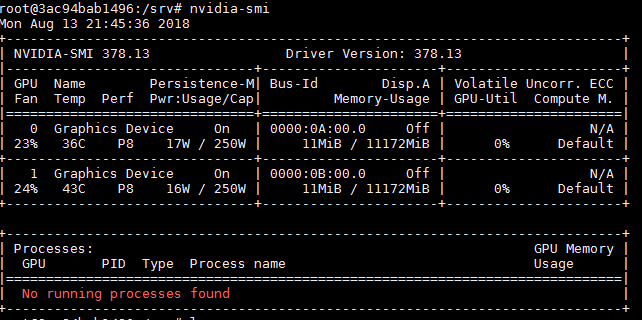
\includegraphics[width=10cm, height=5cm]{./images/gpu_1.PNG}


\raggedright
Running a model on both and checking GPU usage.

\centering
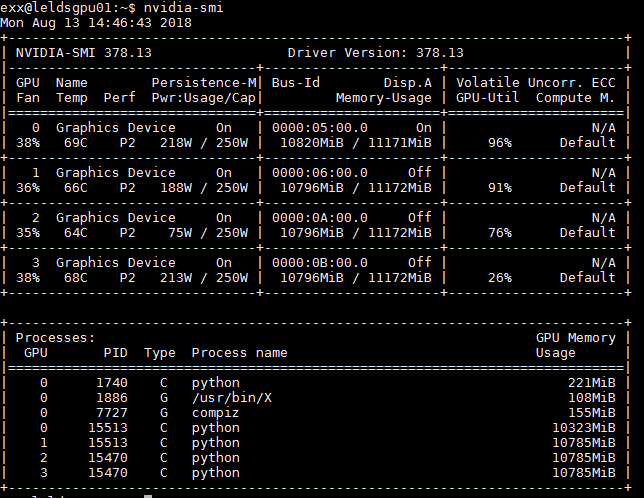
\includegraphics[width=10cm, height=7cm]{./images/usage.PNG}




\raggedright
\subsection{Installation during Docker session}
\small{\begin{tabular} { >{\ttfamily}l  }
pip install --trusted-host pypi.org --trusted-host files.pythonhosted.org \\ --upgrade pip\\
pip install --trusted-host pypi.org --trusted-host files.pythonhosted.org \\ --upgrade tensorflow==1.4.0\\
pip install --trusted-host pypi.org --trusted-host files.pythonhosted.org \\ --upgrade tensorflow-gpu==1.4.0\\
pip uninstall tensorflow\\
pip uninstall tensorflow-gpu\\
pip install --trusted-host pypi.org --trusted-host files.pythonhosted.org \\ --upgrade --force-reinstall tensorflow-gpu==1.4.0\\
pip install --trusted-host pypi.org --trusted-host files.pythonhosted.org \\ --upgrade keras\\
pip install --trusted-host pypi.org --trusted-host files.pythonhosted.org \\ --upgrade theano\\
pip install --trusted-host pypi.org --trusted-host files.pythonhosted.org \\ --upgrade torch\\
pip install --trusted-host pypi.org --trusted-host files.pythonhosted.org \\ --upgrade dlib\\
pip install --trusted-host pypi.org --trusted-host files.pythonhosted.org \\ --upgrade scikit-image\\
pip install --trusted-host pypi.org --trusted-host files.pythonhosted.org \\ --upgrade Cython\\
pip install --trusted-host pypi.org --trusted-host files.pythonhosted.org \\ --upgrade torchvision\\
\end{tabular}
}


\subsection{Commands}

\subsubsection{Used in Tutorial}
\tiny{\begin{tabular} { >{\ttfamily}l  }

\# List current images\\
sudo docker images\\
\\
\# List containers running\\
sudo docker ps\\
\\
\# List containers running history\\
sudo docker ps -a\\
\\
\# Download a given image from Docker Hub\\
sudo docker pull \\
\\
\# To search for docker images\\
https://hub.docker.com/explore/\\
\\
\# Container vs Image \\
\# Using OOPs concepts\\
\# Images: Classes ::: Containers: Objects\\
\#\\
\# Create a new container\\
docker run deep\_learning\_3.0\\
\\
\# Start an existing container\\
docker start CONTAINER\_ID\\
docker stop CONTAINER\_ID\\
\\
\# Remove a Container\\
docker rm CONTAINER\_ID\\
\\
\# Remove an Image\_ID\\
docker rmi IMAGE\_ID\\
\\
\# Update \\
apt-get update\\
\\
\# Setup Proxy\\
export http\_proxy=http://xyz.com:80\\
export https\_proxy=https://xyz.com:80\\
set http\_proxy=http://xyz.com:80\\
set https\_proxy=https://xyz.com:80\\
\\
\# Install Open-CV\\
apt-get install python-opencv\\
\\
\# Test Open CV\\
import cv2\\
\\
\# pip install using trusted host\\
pip install --trusted-host pypi.org --trusted-host files.pythonhosted.org --upgrade pip\\
\\
\\
\# Start docker sharing mount\\
\# -v /local/shared/folder:/shared/folder/in/container/\\
sudo nvidia-docker run -it -v /datafolder/keras/gpu:/srv deep\_learning\_2.0 nvidia-smi\\
\\
\# Port mount docker (Tensorboard 6006)\\
\# -p <host-port>:<container-port>\\
sudo nvidia-docker run -p 6006:6006 deep\_learning\_2.0 nvidia-smi\\
\\
\# Multi - GPU Sharing\\
\# NVIDIA VISIBLE DEVICES PCI/UUID \\
\# Using all 4 GPU\\
sudo nvidia-docker run --runtime=nvidia -e NVIDIA\_VISIBLE\_DEVICES=0,1,2,3 deep\_learning\_2.0 bash\\
\\
\# Split in two\\
sudo nvidia-docker run --runtime=nvidia -e NVIDIA\_VISIBLE\_DEVICES=0,1 deep\_learning\_2.0 nvidia-smi\\
sudo nvidia-docker run --runtime=nvidia -e NVIDIA\_VISIBLE\_DEVICES=2,3 deep\_learning\_2.0 nvidia-smi\\
\\
\# Possible Values:\\
0,1,2,. : a comma-separated list of GPU UUID(s) or index(es).\\
all: all GPUs will be accessible, this is the default value in our container images.\\
none: no GPU will be accessible, but driver capabilities will be enabled.\\
\\
\# Commit Changes and create a new image\\
docker commit CONTAINER\_ID image\_name\\
\# You can also overwite existing Docker Image\\
\\
\# Push to Docker Hub\\
\# Configure Dockerfile\\
docker push user\_name/image\_name\\
\# https://hub.docker.com/\\

	\end{tabular}
}
\subsubsection{From Document}
\small {
\begin{tabular} { >{\ttfamily}l  p{10cm} }
\textbf{Commands:} & \\
	attach    &  Attach local standard input, output, and error streams to a running container \\
	build     &  Build an image from a Dockerfile \\
	commit    &  Create a new image from a container's changes \\
	cp        &  Copy files/folders between a container and the local filesystem \\
	create    &  Create a new container \\
	diff      &  Inspect changes to files or directories on a container's filesystem \\
	events    &  Get real time events from the server \\
	exec      &  Run a command in a running container \\
	export    &  Export a container's filesystem as a tar archive \\
	history   &  Show the history of an image \\
	images    &  List images \\
	import    &  Import the contents from a tarball to create a filesystem image \\
	info      &  Display system-wide information \\
	inspect   &  Return low-level information on Docker objects \\
	kill      &  Kill one or more running containers \\
	load      &  Load an image from a tar archive or STDIN \\
	login     &  Log in to a Docker registry \\
	logout    &  Log out from a Docker registry \\
	logs      &  Fetch the logs of a container \\
	pause     &  Pause all processes within one or more containers \\
	port      &  List port mappings or a specific mapping for the container \\
	ps        &  List containers \\
	pull      &  Pull an image or a repository from a registry \\
	push      &  Push an image or a repository to a registry \\
	rename    &  Rename a container \\
	restart   &  Restart one or more containers \\
	rm        &  Remove one or more containers \\
	rmi       &  Remove one or more images \\
	run       &  Run a command in a new container \\
	save      &  Save one or more images to a tar archive (streamed to STDOUT by default) \\
	search    &  Search the Docker Hub for images \\
	start     &  Start one or more stopped containers \\
	stats     &  Display a live stream of container(s) resource usage statistics \\
	stop      &  Stop one or more running containers \\
	tag       &  Create a tag TARGET\_IMAGE that refers to SOURCE\_IMAGE \\
	top       &  Display the running processes of a container \\
	unpause   &  Unpause all processes within one or more containers \\
	update    &  Update configuration of one or more containers \\
	version   &  Show the Docker version information \\
	wait      &  Block until one or more containers stop, then print their exit codes \\
\end{tabular}



\begin{tabular} { >{\ttfamily}l  p{9cm} }
\textbf{Management Commands:} & \\
config    &  Manage Docker configs \\
container &  Manage containers \\
image     &  Manage images \\
network   &  Manage networks \\
node      &  Manage Swarm nodes \\
plugin    &  Manage plugins \\
secret    &  Manage Docker secrets \\
service   &  Manage services \\
swarm     &  Manage Swarm \\
system    &  Manage Docker \\
trust     &  Manage trust on Docker images \\
volume    &  Manage volumes \\

\end{tabular}




}

\end{document}
